\section{Conjugated segments and rigid fragments}
\label{sec:segments}

\begin{figure}
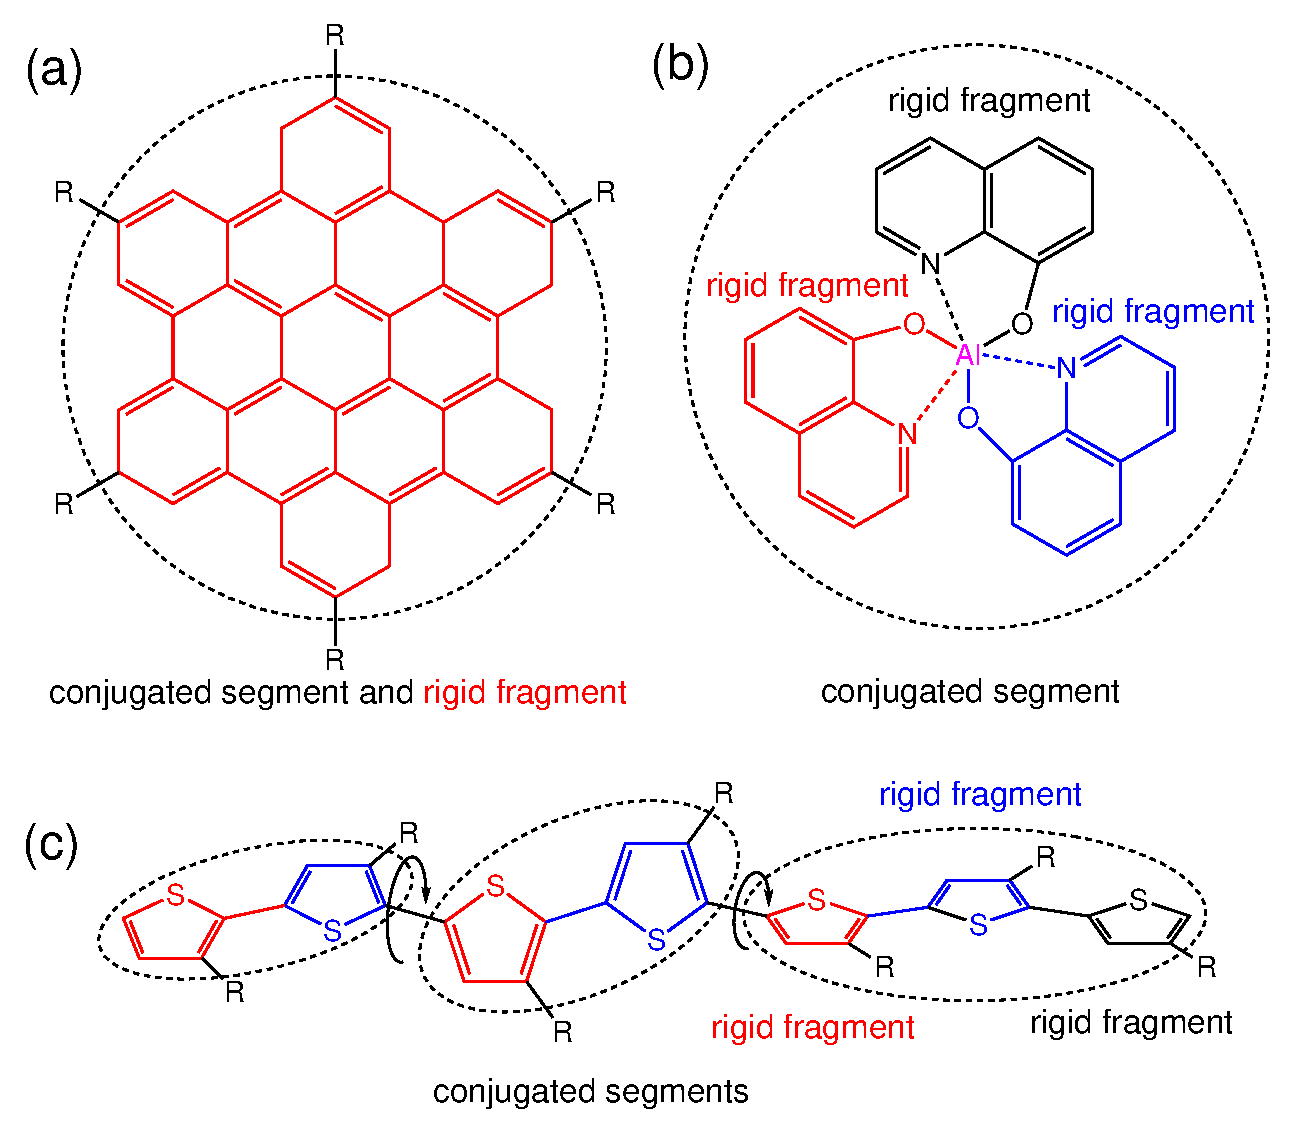
\includegraphics[width=\linewidth]{fig/conjugated_segment/fragment_segment}
\caption{The concept of conjugated segments and rigid fragments. Dashed lines indicate conjugated segments while colors denote rigid fragments. (a) Hexabenzocoronene: the $\pi$-conjugated system is both a rigid fragment and a conjugated segment. (b) \Alq: the Al atom and each ligand are rigid fragments while the whole molecule is a conjugated segment. (c) Polythiophene: each repeat unit is a rigid fragment. A conjugated segment consists of one or more rigid fragments. One molecule can have several conjugated segments.}
\label{fig:segment}
\end{figure}

With the morphology at hand, the next step is partitioning the system on hopping sites\index{hopping site}, or conjugated segments\index{conjugated segment}, and calculating charge transfer rates between them. Physically intuitive arguments can be used for the partitioning,  which reflects the localization of the wave function of a charge. For most organic semiconductors, the molecular architecture includes relatively rigid, planar $\pi$-conjugated systems, which we will refer to as rigid fragments. A conjugated segment can contain one or more of such rigid fragments, which are linked by bonded degrees of freedom. The dynamics of these degrees of freedom evolves on timescales much slower than the frequency of the internal promoting mode. In some cases, e.g. glasses, it can be `frozen' due to non-bonded interactions with the surrounding molecules.

To illustrate the concept of conjugated segments and rigid fragments, three representative molecular architectures are shown in \fig{segment}. The first one is a typical discotic liquid crystal, hexabenzocoronene. It consists of a conjugated core to which side chains are attached to aid self-assembly and solution processing. In this case the orbitals localized on side chains do not participate in charge transport and the conjugated $\pi$-system is both, a rigid fragment and a conjugated segment. 
%
In \Alq, a metal-coordinated compound, a charge carrier is delocalized over all three ligands. Hence, the whole molecule is one conjugated segment. Individual ligands are relatively rigid, while energies of the order of $k_\text{B}T$ are sufficient to reorient them with respect to each other. Thus the Al atom and the three ligands are rigid fragments.
%
In the case of a conjugated polymer, one molecule can consist of several conjugated segments, while each backbone repeat unit is a rigid fragment. Since the conjugation along the backbone can be broken due to large out-of-plane twists between two repeat units, an empirical criterion, based on the dihedral angle, can be used to partition the backbone on conjugated segments~\cite{ruhle_multiscale_2010}. However, such intuitive partitioning is, to some extent, arbitrary and shall be validated by other methods~\cite{vukmirovic_charge_2008,vukmirovic_charge_2009,mcmahon_ad_2009}. 

After partitioning, an additional step is often required to remove bond length fluctuations introduced by molecular dynamics simulations, since they are already integrated out in the derivation of the rate expression. This is achieved by substituting respective molecular fragments with  rigid, planar $\pi$-systems\index{rigid fragment} optimized using first-principles methods. Centers of mass and gyration tensors are used to align rigid fragments, though a custom definition of local axes is also possible. Such a procedure also minimizes discrepancies between the force-field and first-principles-based ground state geometries of conjugated segments, which might be important for calculations of electronic couplings, reorganization energies, and intramolecular driving forces. 

To partition the system on hopping sites and substitute rigid fragments with the corresponding ground-state geometries \xtpmap program is used:
\votcacommand{Mapping the \gromacs trajectory}{\cmdmap}
It reads in the \gromacs topology (\topology) and trajectory (\trajectory) files, definitions of conjugated segments and rigid fragments (\xmlcsg) and outputs coordinates of conjugated segments (hopping sites) and rigid fragments (as provided in the MD trajectory and after rigidification) to the  state file (\sqlstate). In order to do this, a mapping file \xmlcsg has to be provided, which specifies the corresponding atoms in the different representations. After this step, all information (frame number, dimensions of the simulation box, etc) are stored in the \slink{statefile}{state file} and only this file is used for further calculations.

\attention{\votcaxtp requires a wrapped trajectory for mapping the segments and fragments, so all molecules should be whole in the frame.}   

In order to visually check the mapping one can use either the \calc{tdump} \calculator or the programm \xtpdump with the calculator \calc{trajectory2pdb}.

\label{sec:xtp_dump}
\votcacommand{Writing a mapped trajectroy with \xtpdump}{\small \xtpdump \sql \sqlstate \exe \calc{trajectory2pdb} }

It reads in the state file created by \xtpmap and outputs two trajectory files corresponding to the original and rigidified atom coordinates. To check the mapping, it is useful to superimpose the three outputs (original atomistic, atomistic stored in the state file, and rigidified according to ground state geometries), e.g., with {\tt VMD}.

\label{sec:tdump}
\votcacommand{Writing a mapped trajectroy with \calc{tdump} }{\small \xtprun \sql \sqlstate \opt \xmloptions \exe \calc{tdump} }

It also reads in the state file but appends the coordinates to a pdb. file. So make sure to delete old QM.pdb and MD.pdb if you want to create a new imagef


